\documentclass[tikz,border=3pt]{standalone}
\usepackage{amsmath,amssymb}
\usetikzlibrary{arrows.meta,calc}
\definecolor{curveblue}{HTML}{245C86}
\definecolor{accent}{HTML}{A65E2E}
\definecolor{curveteal}{HTML}{287B6D}
\definecolor{curveviolet}{HTML}{76578B}
\begin{document}
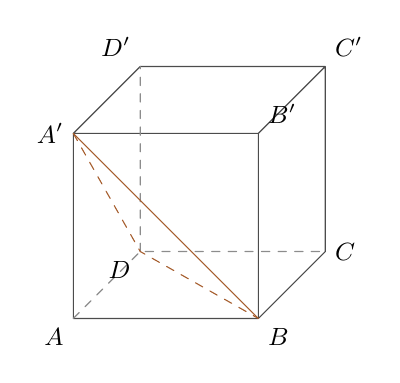
\begin{tikzpicture}[font=\small,>=Latex,line cap=round,line join=round]

\coordinate (A) at (0,0); \coordinate (B) at (2.35,0);
\coordinate (C) at (3.2,.85); \coordinate (D) at (.85,.85);
\coordinate (Ap) at (0,2.35); \coordinate (Bp) at (2.35,2.35);
\coordinate (Cp) at (3.2,3.2); \coordinate (Dp) at (.85,3.2);
\draw[black!70] (A)--(B)--(C)--(Cp)--(Dp)--(Ap)--cycle
    (Ap)--(Bp)--(Cp) (B)--(Bp);
\draw[black!45,dashed] (A)--(D)--(C) (D)--(Dp);
\draw[accent] (Ap)--(B);
\draw[accent,dashed] (Ap)--(D)--(B);
\node[below left] at (A) {$A$};\node[below right] at (B) {$B$};
\node[right] at (C) {$C$};\node[below left] at (D) {$D$};
\node[left] at (Ap) {$A'$};\node[above right] at (Bp) {$B'$};
\node[above right] at (Cp) {$C'$};\node[above left] at (Dp) {$D'$};
\end{tikzpicture}
\end{document}
